

\subsection{Processing Illusion (PIL)}
\label{sc-pil}




\def \fgw {1.05in}


\begin{figure*}[t]

\centerline{
%\includegraphics[height=\fgw]{F/empty.eps}
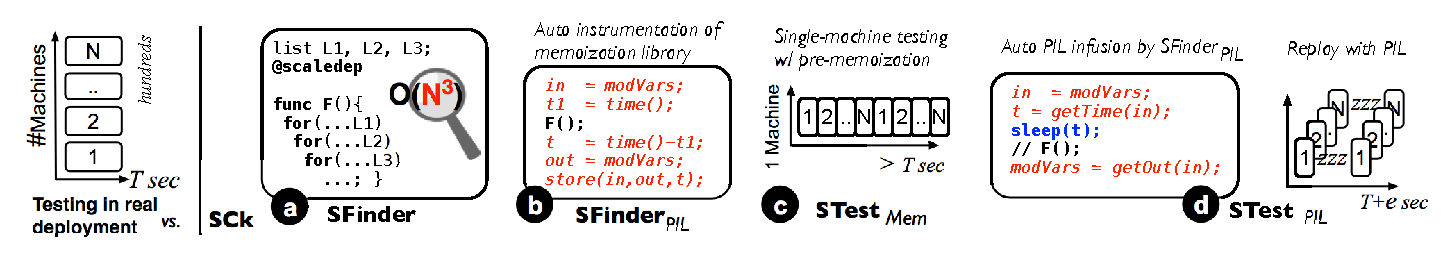
\includegraphics[height=\fgw]{F/ill/sck2.eps}
}

\mycaption{fig-sck}{The complete flow of automation in \sck}{The
left-most figure illustrates testing in real-deployment, where testing
time is fast ($T$) but requires $N$ machines.
%
Stages (a) to (d) reflect the automated \sck process as described
in Section \ref{sc-summ}.
%
\stestm in stage (c) runs on one machine but will take some time
($>$$T$).
%
\stestp in stage (d) still runs on one machine but only consumes
a similar time as in deployment testing ($T$$+$$e$) and can be replayed
numerous times. }


\end{figure*}



% background
Finally, the last challenge we address is: how to produce accurate results
(\ie, the same bug symptoms observed in real-scale deployment) when
colocating hundreds of CPU-intensive nodes on one machine?
%
We found that \stest is sufficient to accurately reveal bug symptoms from
scale-dependent lock-related loops or IO serializations, as these root
causes do not contend for CPUs.
%
For CPU-intensive loops, \stest is also sufficient for master-worker
architecture such as HDFS where only one node (the master) is CPU
intensive.


% background
However, for CPU-intensive loops in P2P systems such as Cassandra, where
{\em all} nodes are busy, the bug symptoms reported by \stest are not
accurate.
%
For example, in \caone (Figures~\ref{fig-mot} and~\ref{fig-code}), in
256-node real deployment, we observe 1948 flappings (the bug symptom),
however, in \stest, we observe 21575 flappings.
%
Similarly in 256-node Riak (\riakone), in a real deployment, the
rebalance duration (the symptom) takes about 8600 seconds, but \stest
reports 22000 seconds.
%
The inaccuracy gets worse as we scale out; with $N$ CPU-intensive nodes on
a $C$-core machine, roughly $N/C$ nodes contend on a given core.



% PIL
To address this, we need to emulate CPU-intensive processing by extending
\stest with {\em processing illusion} (PIL), an approach that replaces an
actual processing with \sleep.  For example, in \caone, we can replace the
expensive gossip/stage-changes processing with \ts{sleep(t)} where \ts{t}
is an accurate timing of how long the processing takes.
%
The intuition behind PIL is similar to the intuition behind other
emulation techniques.
%
For example, Exalt \cite{Wang+14-Exalt} (more in \sec\ref{sec-rel})
provides an illusion of storage space; their insight was ``how data is
processed is not affected by the content of the data being written, but
only by its size.''
%
Similarly, PIL provides an illusion of compute processing; our insight is
that {\em ``the key to computation is not the intermediate results, but
  rather the execution time and eventual output.''}
%
In other words, with PIL, we will still observe the overall timing
behaviors and the corresponding impacts accurately.



% intro to PIL
PIL might sound outrageous initially, but it is feasible as we
address the two following concerns:
%
how a function (or code block) can be safely replaced with \sleep
\textit{without} changing the whole processing semantic
(\sec\ref{sc-pil-1}) and
%
how we can produce the output and predict the timing
``\ts{t}'' if the actual compute is skipped (\sec\ref{sc-pil-2}).




% -----------------------------------
\subsubsection{PIL-Safe Functions}
\label{sc-pil-1}

Our first challenge is to ensure that functions (or code blocks) can be
safely replaced with \sleep, but still retain the cluster-wide behavior
and unearth the bug symptoms.  We name such functions as {\em PIL-safe
  functions}.
%
We identify two main characteristics of sleep-safe functions:
% by memoization
(1) Memoizable output: a PIL-safe function must have a memoizable
(deterministic) output based on the input of the function.
% ...
(2) Non-pertinent I/Os: if a function performs disk/network I/Os that are
not pertinent to the correctness of the corresponding protocol, the
function is PIL-safe.  For example, in \caone, there is a ring-table
checkpoint (not shown) needed for fault tolerance but is irrelevant (never
read) during bootstrapping.
%
We extend \sfind to \sfindp, which includes a static analysis that finds
code blocks in scale-dependent loops that can be safely PIL-ed.

% In our experience, all of them can be PIL-ed and still lead to a correct
% completion.



% -----------------------------------
\subsubsection{Pre-Memoization (with Order Determinism)}
\label{sc-pil-2}


As PIL-safe functions no longer perform the actual computation, the next
question to address is: how do we manufacture the output such that the
global behavior is not altered (\eg, rebalancing protocol should terminate
successfully)?
%
Our solution is {\em pre-memoization}, which records input-output pairs
and the processing time, specifically a tuple of three items
(\ts{ByteString} \ts{in}, \ts{out}, \ts{long} \ts{nanoSec}) indexed by
\ts{hash(in)}), which represent the to-be-modified variables before and
after the function is executed and the processing time, respectively, as
illustrated in Figure \ref{fig-sck}b.
%
We extend \sfindp to {\em automatically} instrument the target code and insert
our pre-memoization libraries around the PIL-safe function.


Another challenge we encountered is non-determinism: the state of each
node (the input) depends on the order in which messages arrive (which are
typically random).
%
To address this, during pre-memoization, we also record non-deterministic
events such as message orderings such that order determinism is enforced
during replays \cite{Geels+07-Friday}.
% \stestm (akin to deterministic record and replay




% Gautam+09-ODR,   Geels+06-Liblog, Guo+08-R2, Soyeon+09-PRES



